The surficial carbon cycle and solid-Earth carbon cycle operate on two different time scales. ~\cite{HRA:2007} considered the short-term carbon budget in the surficial reservoirs: atmosphere, oceans, terrestrial ecosystems and fossil fuels over the time period of years to centuries. The annual transport of carbon due to processes such as weathering, and volcanism are small. However, these processes are dominant on the time scale of millennia. ~\citet{SNH-ZK:2001} constructed a simple carbon reservoir model that spanned from the Archean to present day. Their reservoir model consisted of the following reservoirs: continental sediments, ocean, oceanic crust, and mantle. Below is an overview of carbon in the different reservoirs and their relevant fluxes during the long-term carbon cycle.

On the time scale of millions of years, two important components of the carbon cycle includes the crustal Urey cycle and the mantle cycle. The crustal Urey cycle is a closed cycle including silicate weathering and metamorphism of carbonates. The Urey reaction is 

\begin{equation}
\label{EQ:Urey_reaction}
  \text{CO}_2 + \text{CaSiO}_3 \rightleftharpoons \text{CaCO}_3 + \text{SiO}_2.
\end{equation}

\noindent Exposed $\mathrm{Ca}^{2+}$ or $\mathrm{Mg}^{2+}$ silicate bearing rocks in the continental crust undergo weathering from dissolved carbon in acidic rainfall. The resulting cations and anions are transported to the oceans by river systems where both organic and inorganic precipitation of $\text{CaCO}_3$ occurs. The crustal Urey cycle is closed due to carbonate metamorphism resulting in degassing of carbon dioxide through subduction zone volcanism ~\cite{KLH-TDL-WM:2017}. The reaction rate of the Urey reaction is dependent on the concentration of $\text{CO}_2$ and temperature in the atmosphere, changing sea levels and rainfall.

In the mantle cycle, an influx of carbonates through subduction is offset by the outflux of $\text{CO}_2$ through mid-ocean ridge and island-arc volcanism.  Accumulated pelagic carbonates on seafloors and carbonatized basaltic crust are subducted over time. A portion of the subducting material is transported to the atmosphere by island arc volcanism where as the remainder is transported into the mantle. ~\citet{SNH-ZK:2001} estimates the residence time of carbon in the atmosphere and mantle to be 1 Kyr and 7.2 Myr respectively. Mid-ocean ridge volcanism and ocean-island volcanism sample the heterogeneous mantle transporting carbon from the deep interior to the surficial reservoirs. Due to decay rate of plate tectonics, the rate of subduction and volcanism are temporally evolving.

A large fraction of Earth's carbon inventory resides within the core. ~\cite{DR-CH-SN:2013} estimates the mass of carbon in the core to be $4.44 \times 10^9$ Gt ($1~\text{Gt} = 10^{12}$ Kg). However, since the giant moon-forming impact, there is little to no evidence of the exchange of carbon from the core to the mantle and is therefore often considered an isolated reservoir. 

A comprehensive reservoir model of Earth's carbon cycle today is shown in Fig.~\ref{FIG:SNHZKBoxModelDiagram}. Estimates for the masses of carbon in Earth's major carbon reservoirs are shown in Table.~\ref{Table:Masses of carbon in Earth's reservoirs}. Error bars are not include because the uncertainties are difficult to specify.

\begin{figure}[h!]
  \centering
  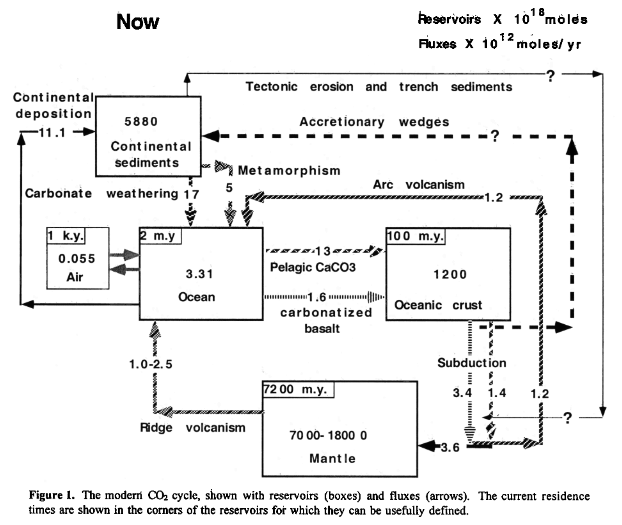
\includegraphics[scale=0.5]{Figures/SNH-ZK-2001_BoxModelDiagram.png}
  \label{FIG:SNHZKBoxModelDiagram}
  \caption{A comprehensive reservoir model of carbon cycle proposed by ~\citet{SNH-ZK:2001}}
\end{figure}

%Although the atmosphere presently contains a small fraction of Earth's carbon inventory, ~\citet{KJD:2002} suggests the possibility of a significant fraction of Earth;s initial carbon inventory residing in the atmosphere. Scaling the carbon concentration of Venusian atmosphere to that of Earth's atmosphere based on their mass ratios, gives an estimated value of carbon in Earth's early atmosphere is $^cM_a(t_0) = 1.28 \time 10^8$ Gt. Alternatively, Earth's early atmosphere may have resembled today's atmosphere with an estimated value of carbon presently is $^cM_a(t_0) =\, ^cM_a(t_p) = 8.5 \times 10^2$ Gt ~\cite{NOAA:2017}. In both cases, Urey reaction plays an important role by transferring carbon from the atmosphere into the oceans where calcium carbonates precipitate ~\cite{UHC:1952}. 





% which was subsequently drawn down until cooling of global magma ocean and then further drawn down as the continental crust was being built. ~\citet{KJD:2002} estimates that this drawdown before reaching quasi-steady state could of been completed by the end of Archean or 1.5Ga ago at the latest. Alternatively, the atmosphere may have contained only a small fraction of the Earth;s carbon inventory thoughout its history with the Urey reaction as an important controlling process on the flux rate of carbon from the atmosphere to the continental crust. The source of the carbon in this model is associated with the mantle due to a higher flux of carbon release from volcanism in comparison to the flux of carbon subducted.